\adparagraph{nDCG}
Figure \ref{fig:ndcg} shows the nDCG score for BC, MC, SF, and Avg. For nDCG a higher score is better as covered in Section \ref{sec:methodology_ndcg}.
All methods see a sharp drop off in the quality of their recommendations as the group sizes increase.
BC drops the most in the jump from 4 to 8 group members, however it also have the best results, and outperforms all other methods across all group sizes.
MC is second best by only a few percentage points and follows the same trend and quickly plateaus in score.
One outlying case SF starts out close to Avg for a group size of four, but retains a higher score and is closer to BC and MC as the size increases.
Avg is the worst performing.

\begin{figure}[H]
	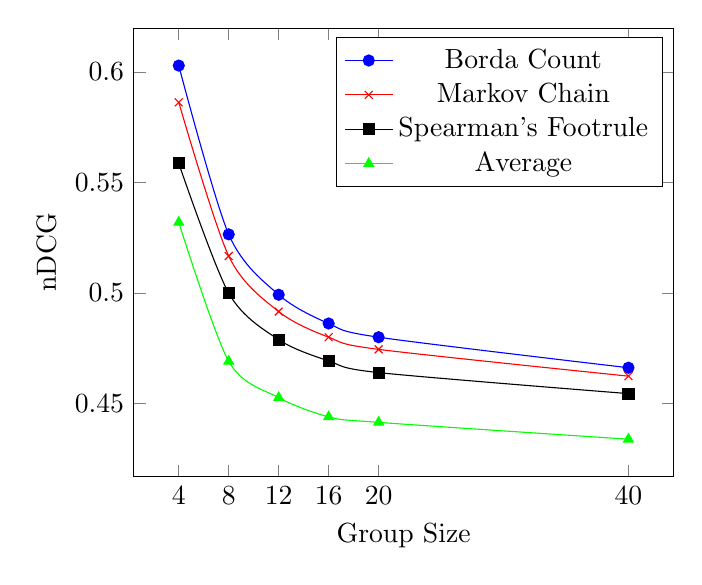
\begin{tikzpicture}
	\begin{axis}[
	xlabel=Group Size,
	ylabel=nDCG,
	xtick = {4,8,12,16,20,40}]
	\addplot[smooth,mark=*,blue] plot coordinates {
		(4,0.6028)
		(8,0.5265)
		(12,0.4992)
		(16,0.4862)
		(20,0.48)
		(40,0.4662)
	};
	\addlegendentry{Borda Count}
	
	\addplot[smooth,color=red,mark=x] plot coordinates {
		(4,0.5862)
		(8,0.5167)
		(12,0.4916)
		(16,0.48)
		(20,0.4745)
		(40,0.4624)
	};
	\addlegendentry{Markov Chain}
	
	\addplot[smooth,color=black,mark=square*] plot coordinates {
		(4,0.5586)
		(8,0.4999)
		(12,0.4789)
		(16,0.4693)
		(20,0.464)
		(40,0.4545)
	};
	\addlegendentry{Spearman's Footrule}
	
	\addplot[smooth,color=green,mark=triangle*] plot coordinates {
		(4,0.5319)
		(8,0.4691)
		(12,0.4527)
		(16,0.444)
		(20,0.4415)
		(40,0.4339)
	};
	\addlegendentry{Average}
	
	\end{axis}
	\end{tikzpicture}
	\caption{Results for nDCG test}\label{fig:ndcg}
\end{figure}